\chapter{Discussion}
\label{chp:discussion}

This chapter discusses the implications of our experimental results and their broader significance for 3D city modelling applications.

\section{Use Cases of FlatCityBuf}
\label{use_case_flat_city_buffer}

This section examines the most appropriate application scenarios for the FlatCityBuf format based on its demonstrated performance characteristics.

\subsection{Flexible Data Download}
\label{flexible_data_download}

Providing users with the ability to download specific data of interest represents one of the most valuable applications of 3D city models, particularly within open data initiatives. Existing services such as 3DBAG offer download functionality for CityJSON data in various formats including CityJSON, OBJ, and GeoPackage. However, these services typically constrain users to downloading predefined tiles rather than precisely the data matching their specific requirements.

\href{https://fcb-web-prototype.netlify.app}{This web prototype} demonstrates that users can download precisely the data they require. This implementation successfully showcases FlatCityBuf's capability to facilitate targeted data retrieval. Through its attribute indexing mechanism, users can download filtered datasets based on specific criteria, such as features exceeding 100 metres in height.

\subsection{Data Analysis}
\label{data_analysis}

As demonstrated by the performance benchmarks, FlatCityBuf excels in read operations compared to alternative data formats, making it particularly suitable for analysing large-scale datasets. This performance advantage is especially valuable in data processing pipelines where \ac{io} operations constitute a significant bottleneck.

A compelling example is the 3DBAG generation pipeline, which involves multiple stages that require reading and writing CityJSONSeq files. In such workflows, \ac{io} performance directly impacts overall processing time. This efficiency becomes increasingly important when processing large urban datasets containing millions of building features.

The format also simplifies analytical workflows. Conventional approaches to large-scale data processing often require chunking data across multiple files, necessitating additional programming to manage file aggregation. In contrast, FlatCityBuf encapsulates data in a single file that can be efficiently loaded and accessed, even in web-based environments, streamlining analytical processes. This unified approach reduces the complexity of data management while maintaining high performance for both selective queries and full dataset processing.

\section{Impact on Server Architecture}
\label{affect_on_server_architecture}

FlatCityBuf introduces significant opportunities for simplifying server architectures for 3D city model delivery.

\subsection{Traditional Server Architecture}
\label{traditional_server_architecture}

Conventional server architectures for 3D city models typically employ both application and database servers. For example, \citet{3dcitydb} utilises PostgreSQL or Oracle as the database server with PostgREST API \citep{postgrest} providing data access through its toolchain. Similarly, the 3DBAG \ac{api} uses PostgreSQL as its database server and Flask (Python web framework) as the application server.

In contrast, FlatCityBuf operates as a static file, requiring only a basic HTTP server such as Nginx \citep{nginx} for data distribution. This approach aligns with modern cloud service offerings, where providers like AWS S3 \citep{s3} and Google Cloud Storage \citep{gsc} offer optimised solutions for serving static content.

\subsection{Cloud Architecture Advantages}
\label{cloud_architecture_achieved}

\subsubsection{Scalability}
\label{scalability}

Scalability presents a significant challenge in traditional server architectures. These systems typically employ \ac{rdbms} that often encounter scaling limitations. Common mitigation strategies include sharding and replication (horizontal scaling) or resource expansion (vertical scaling), both requiring additional computational, memory, and storage resources.

FlatCityBuf circumvents these challenges by functioning as a static file that can leverage cloud providers' inherent scalability and high availability infrastructure. This characteristic offers substantial benefits for applications built on 3D city model data. Service providers can host static FlatCityBuf files on standard servers, allowing unrestricted access for various use cases without implementing the rate-limiting mechanisms often necessary with traditional server architectures.

\subsubsection{Cost-effectiveness}
\label{cost_effectiveness}

FlatCityBuf contributes significantly to operational cost-effectiveness. Although precise server costs vary according to specific use cases, hosting static files through cloud service providers is generally substantially more economical than maintaining dedicated database and application servers.
For example, Google Cloud's storage service, Cloud Storage, costs \$0.020 USD per GB per month in the Netherlands (europe-west4) region\footnote{Google Cloud Storage Pricing, \url{https://cloud.google.com/storage/pricing\#europe}, accessed January 2025}.
In contrast, computing services such as Compute Engine cost \$0.25 USD per vCPU hour for on-demand instances in the same region (4 vCPU, 16 GiB memory, 375 GiB SSD)\footnote{Google Cloud Compute Engine Pricing, \url{https://cloud.google.com/compute/all-pricing?hl=en}, accessed January 2025}.
While direct cost comparisons between storage and compute services are complex due to their different pricing models, storage services offer inherently unlimited scalability, whereas compute services require provisioning additional server instances to achieve substantial scalability.
This fundamental difference in architecture demonstrates that hosting static files is considerably more cost-effective than traditional server architectures requiring continuous compute resources.

\begin{figure}[htbp]
  \centering
  \begin{subfigure}[b]{0.48\textwidth}
    \centering
    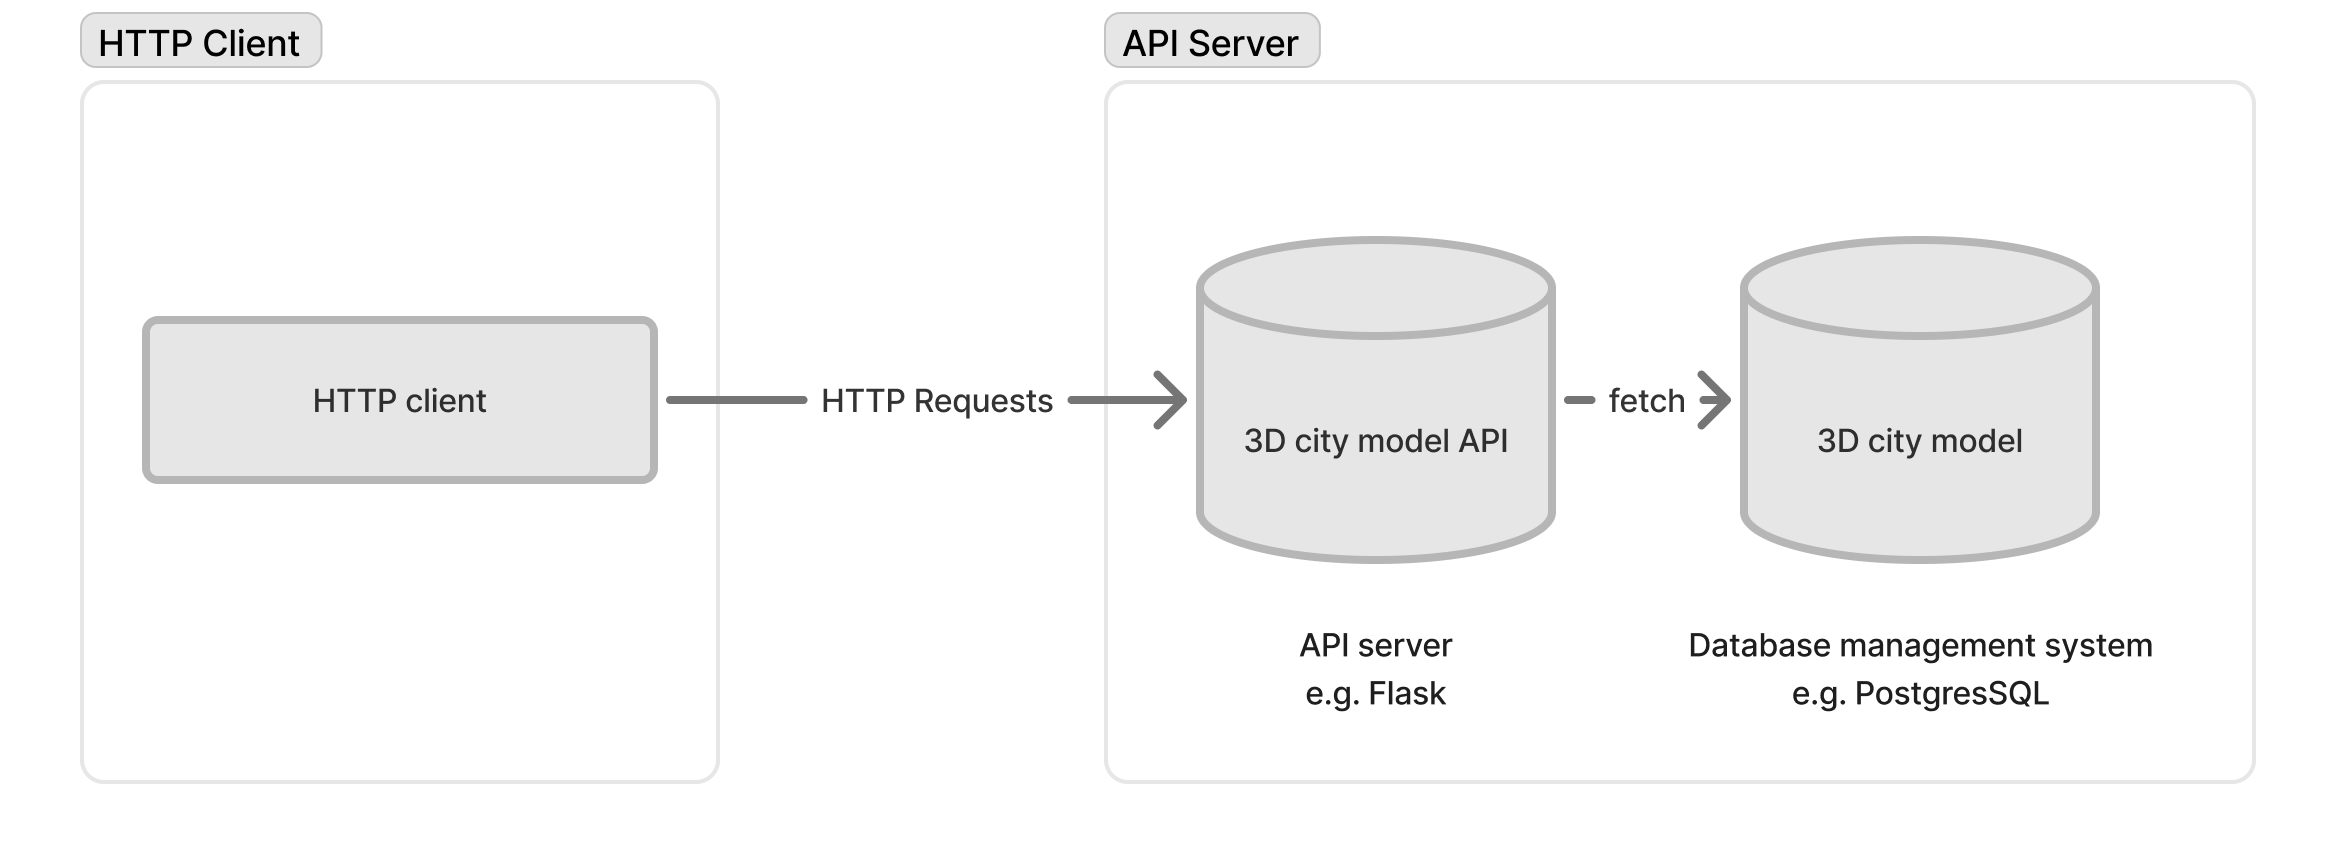
\includegraphics[width=\textwidth]{figs/discussion/server_architecture.png}
    \caption{Traditional server architecture with database and application servers}
    \label{fig:traditional_architecture}
  \end{subfigure}
  \hfill
  \begin{subfigure}[b]{0.48\textwidth}
    \centering
    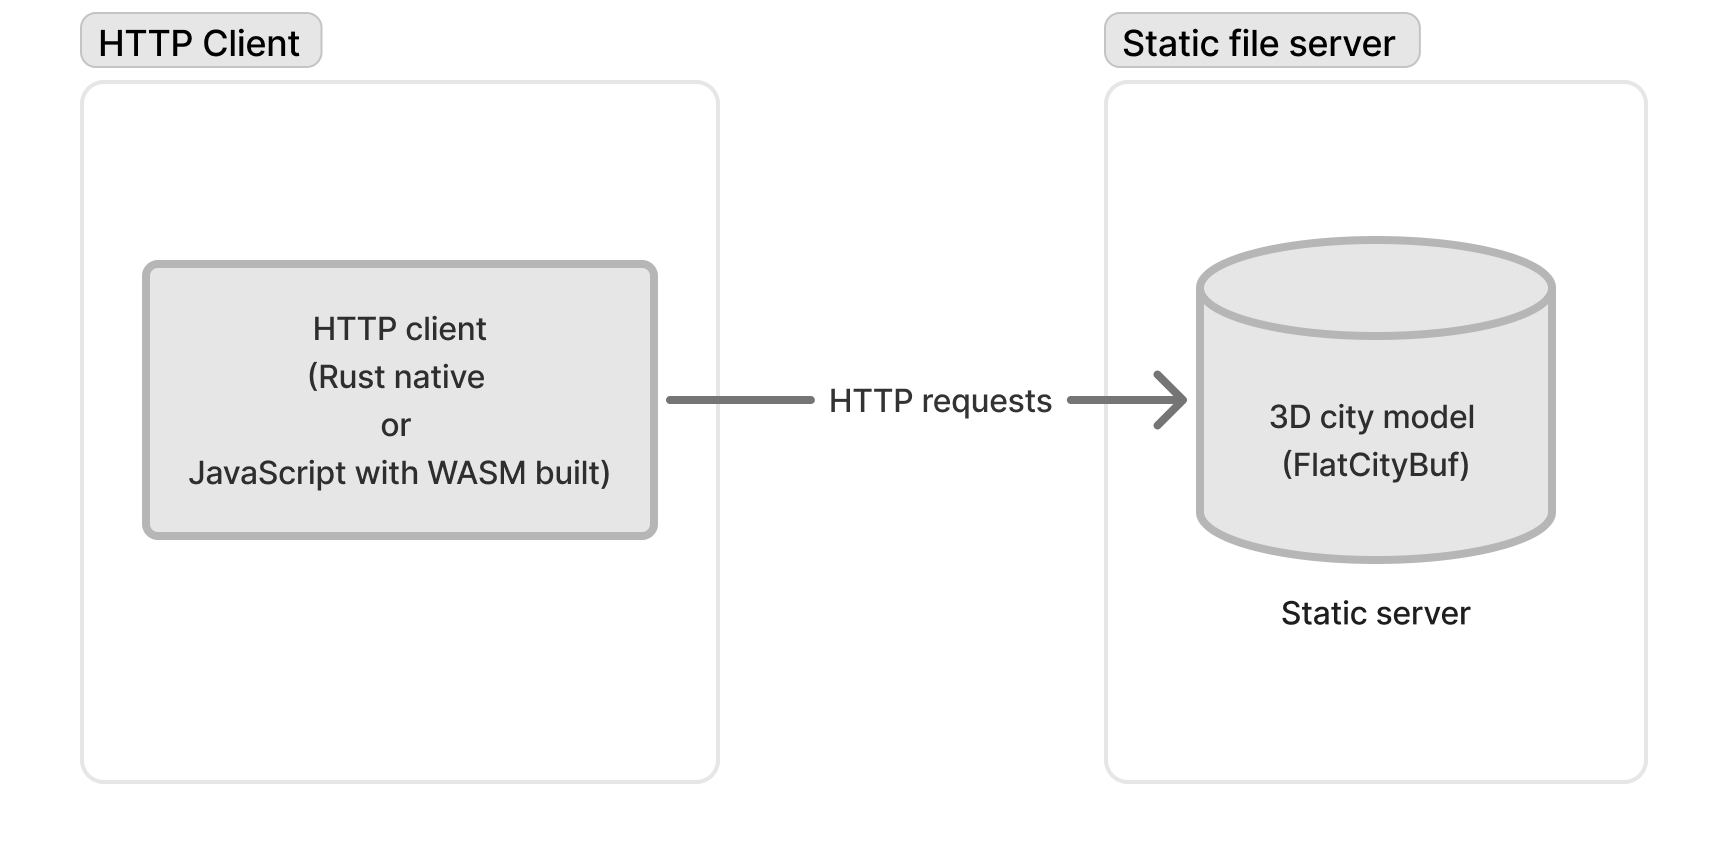
\includegraphics[width=\textwidth]{figs/discussion/server_architecture_fcb.png}
    \caption{Simplified FlatCityBuf architecture}
    \label{fig:fcb_architecture}
  \end{subfigure}
  \caption{Comparison between traditional and FlatCityBuf server architectures. The proposed method eliminates the need for complex database infrastructure by leveraging static file hosting with built-in spatial and attribute indices.}
  \label{fig:architecture_comparison}
\end{figure}

\section{Limitations}
\label{limitations}

Despite its advantages in simplicity, scalability, and cost-effectiveness, FlatCityBuf does present certain limitations that warrant consideration.

\subsection{Query Flexibility}
\label{flexibility_of_query}

While FlatCityBuf supports both spatial and attribute indexing, its query capabilities remain more constrained than those of specialised spatial database applications. Traditional approaches employing \ac{rdbms} with spatial indexing provide more comprehensive query functionality. For instance, 3DCityDB enables filtering by \ac{lod}, CityObject type \citep{3dcitydb}, and various other parameters, whereas FlatCityBuf primarily supports attribute-based filtering. Similarly, regarding spatial functions, 3DCityDB can utilise the extensive spatial capabilities of PostGIS \citep{postgis}, while FlatCityBuf currently only implements bounding box queries, nearest neighbour queries, and point intersection queries. Consequently, FlatCityBuf is optimised for scenarios requiring relatively straightforward filtering conditions.

\subsection{Client-side Application Complexity}
\label{complexity_of_client_side_application}

Although FlatCityBuf simplifies server architecture, it introduces additional complexity in client-side applications, which must implement logic for loading and processing the format. This shift in computational responsibility follows the client-server architecture spectrum described by \citet{alesheikh_2002}, who categorised systems ranging from "Thin Client" (where clients primarily handle display) to "Thick Client" (where clients perform most processing tasks).

Figure \ref{fig:alesheikh_2002_architecture} illustrates the original model proposed by \citet{alesheikh_2002}, while Figure \ref{fig:fcb_thickness} demonstrates where FlatCityBuf fits within this framework. As these figures show, FlatCityBuf represents an extreme case of the "Thick Client" architecture. Since the client assumes responsibility for filtering services in addition to other processing tasks, the complexity exceeds that of traditional architectures where such operations are handled server-side.

This architectural choice has implications for interoperability. OGC API \citep{ogc_api} and equivalent Web \ac{api} services adhere to standardised designs that enable universal client access—whether through command-line interfaces, web browsers, or mobile applications. While FlatCityBuf supports cross-platform deployment, it requires language-specific or platform-specific library implementations, potentially limiting its accessibility compared to standard web APIs.

\begin{figure}[htbp]
  \centering
  \begin{subfigure}[b]{0.45\textwidth}
    \centering
    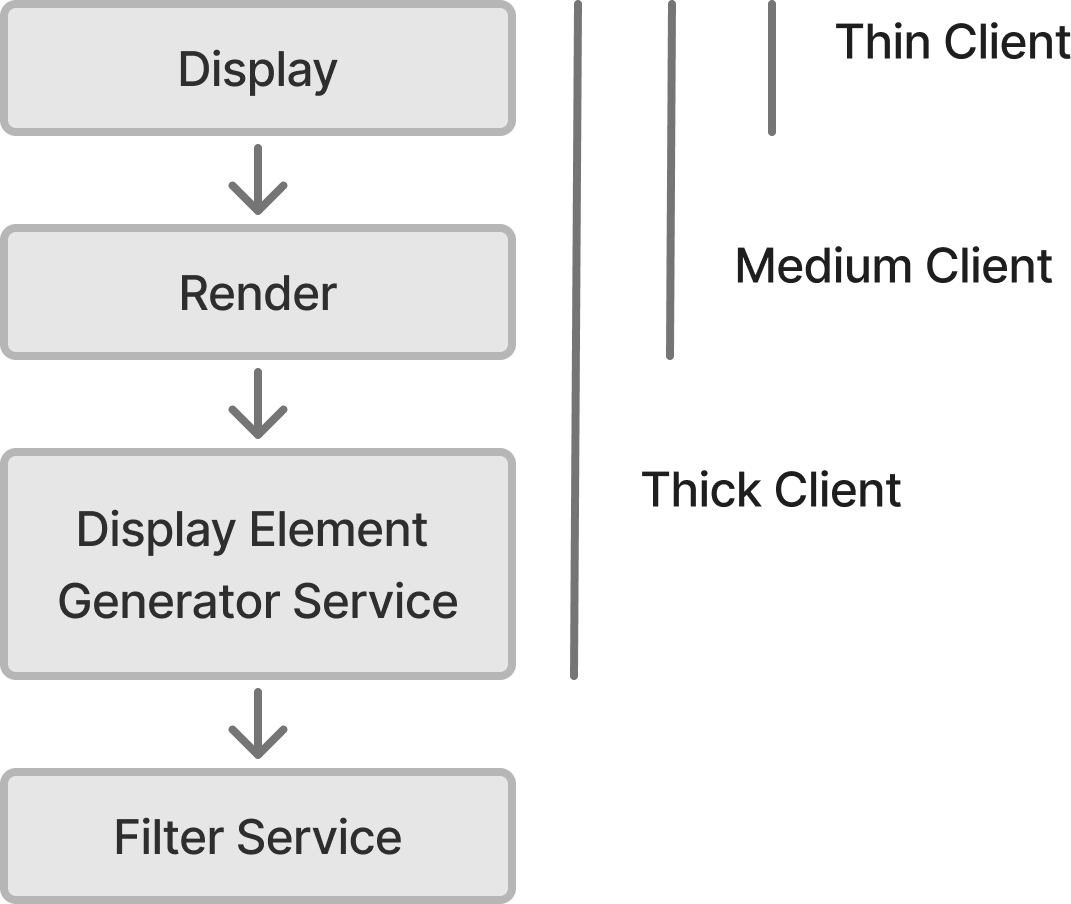
\includegraphics[width=\textwidth]{figs/discussion/client_architecture1.png}
    \caption{Client architecture model modified from \citet{alesheikh_2002}}
    \label{fig:alesheikh_2002_architecture}
  \end{subfigure}
  \hfill
  \begin{subfigure}[b]{0.45\textwidth}
    \centering
    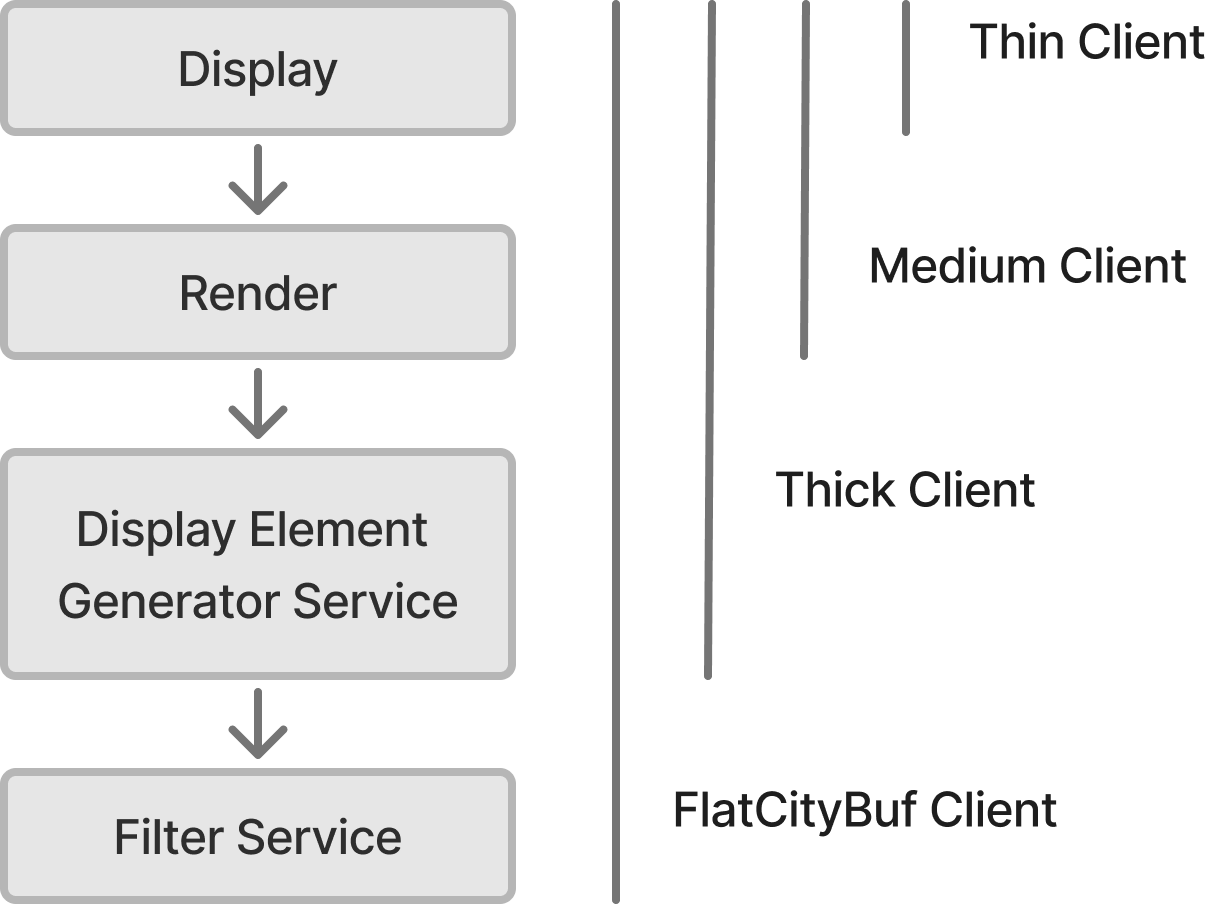
\includegraphics[width=\textwidth]{figs/discussion/client_architecture2.png}
    \caption{FlatCityBuf architecture with \citet{alesheikh_2002}'s model}
    \label{fig:fcb_thickness}
  \end{subfigure}
  \caption{Comparison of client complexity with \citet{alesheikh_2002}'s model and FlatCityBuf's architecture.}
  \label{fig:thickness_of_client}
\end{figure}

\subsection{Update Complexity}
\label{ease_of_update}

Zero-copy data formats like FlatCityBuf generally present challenges for data updates due to their relatively rigid structure. Fixed-size data types such as integers or floating-point numbers cannot be dynamically converted to alternative types. Furthermore, since the format contains immutable spatial and attribute indices, updating the data necessitates rewriting the entire file. This characteristic renders FlatCityBuf less suitable for frequently updated datasets, positioning it instead as an optimal solution for data analysis and efficient download services.
